\begin{solution}
\begin{enumerate}
\item {[4 points]} The best approximation to $f(x) = e^x$ from ${\rm span}\{\phi_1\}$ with respect to the norm $\norm{\cdot}$ is
       \[ f_1(x) = {(f,\phi_1) \over (\phi_1, \phi_1)} \phi_1(x).\]
      We compute
\[
          \ip{\phi_1,\phi_1} = \int_{-1}^1 1^2\,dx = \left[x\right]_{-1}^1=1-\left(-1\right)=2
\]
and
\[
          \ip{f,\phi_1} = \int_{-1}^1 e^x\,dx = \left[e^x\right]_{-1}^1=e^1-e^{-1}=e-{1\over e}
\]
      and hence
       \[ f_1(x) = {1\over 2}\left(e-{1\over e}\right).\]
\\
\item {[7 points]} Since $\phi_1$ and $\phi_2$ are
      orthogonal with respect to the inner product $\ip{\cdot,\cdot}$, i.e., $\ip{\phi_1, \phi_2} = 0$, the best approximation to $f(x) = e^x$ from ${\rm span}\{\phi_1,\phi_2\}$ with respect to the norm $\norm{\cdot}$ is
       \[ f_2(x) = {(f,\phi_1) \over (\phi_1, \phi_1)} \phi_1(x) + {(f,\phi_2) \over (\phi_2, \phi_2)} \phi_2(x) = f_1(x) + {(f,\phi_2) \over (\phi_2, \phi_2)} \phi_2(x).\]
      Noting that
      \[
         \ip{\phi_2,\phi_2} =\int_{-1}^1 x^2\,dx = \left[{x^3\over 3}\right]_{-1}^1 = {1 \over 3} - \left(-{-1 \over 3}\right) = {1 \over 3} - {1 \over 3} = {2\over 3}
\]
and
\[
         \ip{f,\phi_2} =\int_{-1}^1 xe^x\,dx =\left[xe^x\right]_{-1}^1-\int_{-1}^1 e^x\,dx = e^1-\left(-e^{-1}\right)-\ip{f,\phi_1} = e+{1\over e}-e+{1\over e} = {2\over e}
\]
      we can compute that
       \[ f_2(x) = f_1(x)
                  + {(f,\phi_2) \over (\phi_2, \phi_2)} \phi_2(x) = {1\over 2}\left(e-{1\over e}\right)
                  + {3\over e}x.\]
\\
\item {[7 points]}
Since,
 \[ (\phi_1,\phi_2) = (\phi_1,\phi_3) = (\phi_2,\phi_3) = 0,\]
the best approximation to $f(x) = e^x$ from ${\rm span}\{\phi_1,\phi_2,\phi_3\}$ with respect to the norm $\norm{\cdot}$ is
       \[ f_3(x) = {(f,\phi_1) \over (\phi_1, \phi_1)} \phi_1(x) + {(f,\phi_2) \over (\phi_2, \phi_2)} \phi_2(x) + {(f,\phi_3) \over (\phi_3, \phi_3)} \phi_3(x) = f_2(x) + {(f,\phi_3) \over (\phi_3, \phi_3)} \phi_3(x).\]
Toward this end, compute
\begin{eqnarray*}
  \ip{\phi_3,\phi_3} &=& \int_{-1}^1 (3x^2-1)^2\,dx
\\
 &=& \int_{-1}^1 9x^4-6x^2+1\,dx
\\
 &=& \int_{-1}^1 9x^4\,dx-6\ip{\phi_2,\phi_2} +\ip{\phi_1,\phi_1}
\\
 &=& \left[{9x^5\over 5}\right]_{-1}^1-6{2\over 3} +2
\\
 &=& {9\over 5}-\left(-{9\over 5}\right)-{12\over 3} +2
\\
 &=& {18\over 5}-{12\over 3} +2
\\
 &=& {54\over 15}-{60\over 15} +{30\over 15}
\\
 &=& {24\over 15}
\\
 &=& {8\over 5}
\end{eqnarray*}
and
\begin{eqnarray*}
\ip{f,\phi_3} &=& \int_{-1}^1 (3x^2-1)e^x\,dx
\\
&=& \int_{-1}^1 3x^2e^x\,dx-\ip{f,\phi_1}
\\
 &=& \left[3x^2e^x\right]_{-1}^1-\int_{-1}^1 6xe^x\,dx-\left(e-{1\over e}\right)
\\
 &=& 3e^1-3e^{-1}-6\ip{f,\phi_2}-\left(e-{1\over e}\right)
\\
 &=& 2e-{2\over e}-{12\over e}
\\
 &=& 2e-{14\over e}
\end{eqnarray*}
thus giving
       \[ f_3(x) = f_2(x) + {(f,\phi_3) \over (\phi_3, \phi_3)} \phi_3(x) = {1\over 2}\left(e-{1\over e}\right)
                  + {3\over e}x + {5\over 4} \left(e-{7\over e}\right) (3x^2-1) .\]
\\
\item {[7 points]} The following plot compares the best approximations to $f(x)$.

\begin{center} 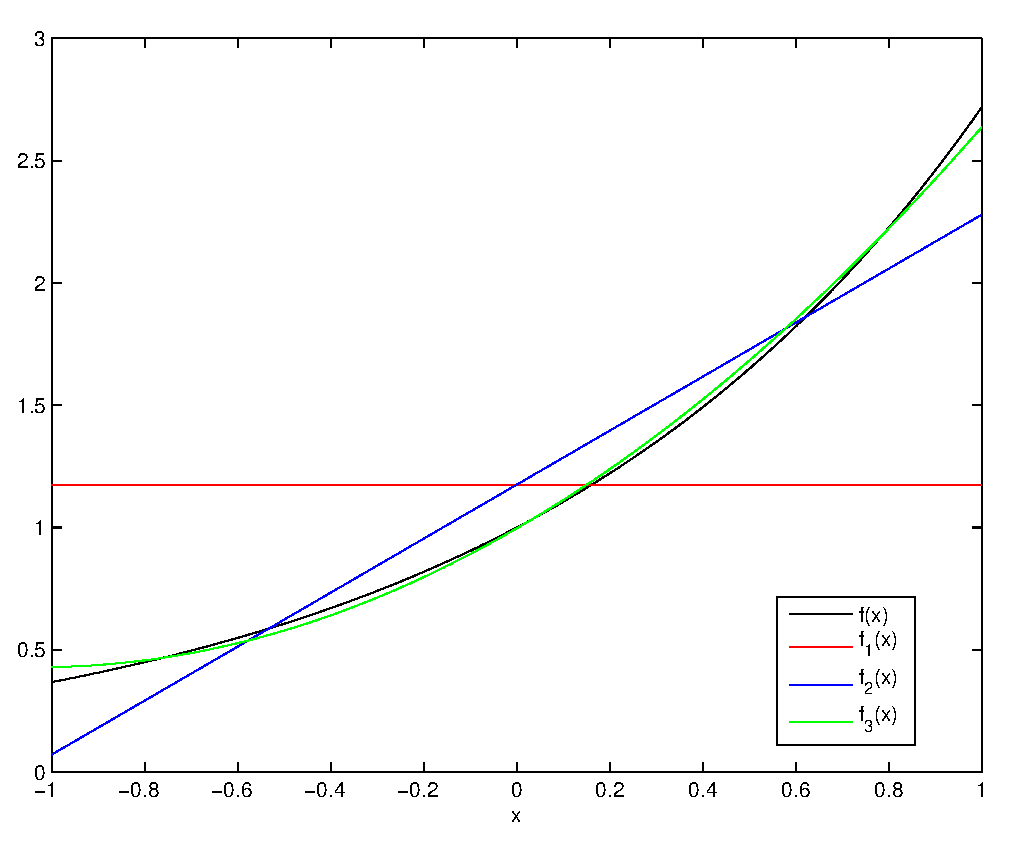
\includegraphics[scale=0.5]{hw16d} \end{center}

The code use to produce it is below.

\lstinputlisting{HW16d.m}
\end{enumerate}
\end{solution}

